\chapter{Project Planning}
\label{planning}
\thispagestyle{plain}

This project is comprised two phases. In the first phase, which is currently completed, consisted on the research of the timetabling problem, with emphases on the ITC 2007 Track 3 Curriculum-Based Timetable problem, and several meta-heuristic algorithms that are used to create automated solvers. In this phase, we also selected the algorithms that will be implemented and defined the way in which the results obtained with each implementation will be analyzed.\\
Figure~\ref{fig:completedTasks} presents the allocation of time to the most relevant tasks were executed in the first phase of this project.\\
\begin{figure}[h!]
 \centering
   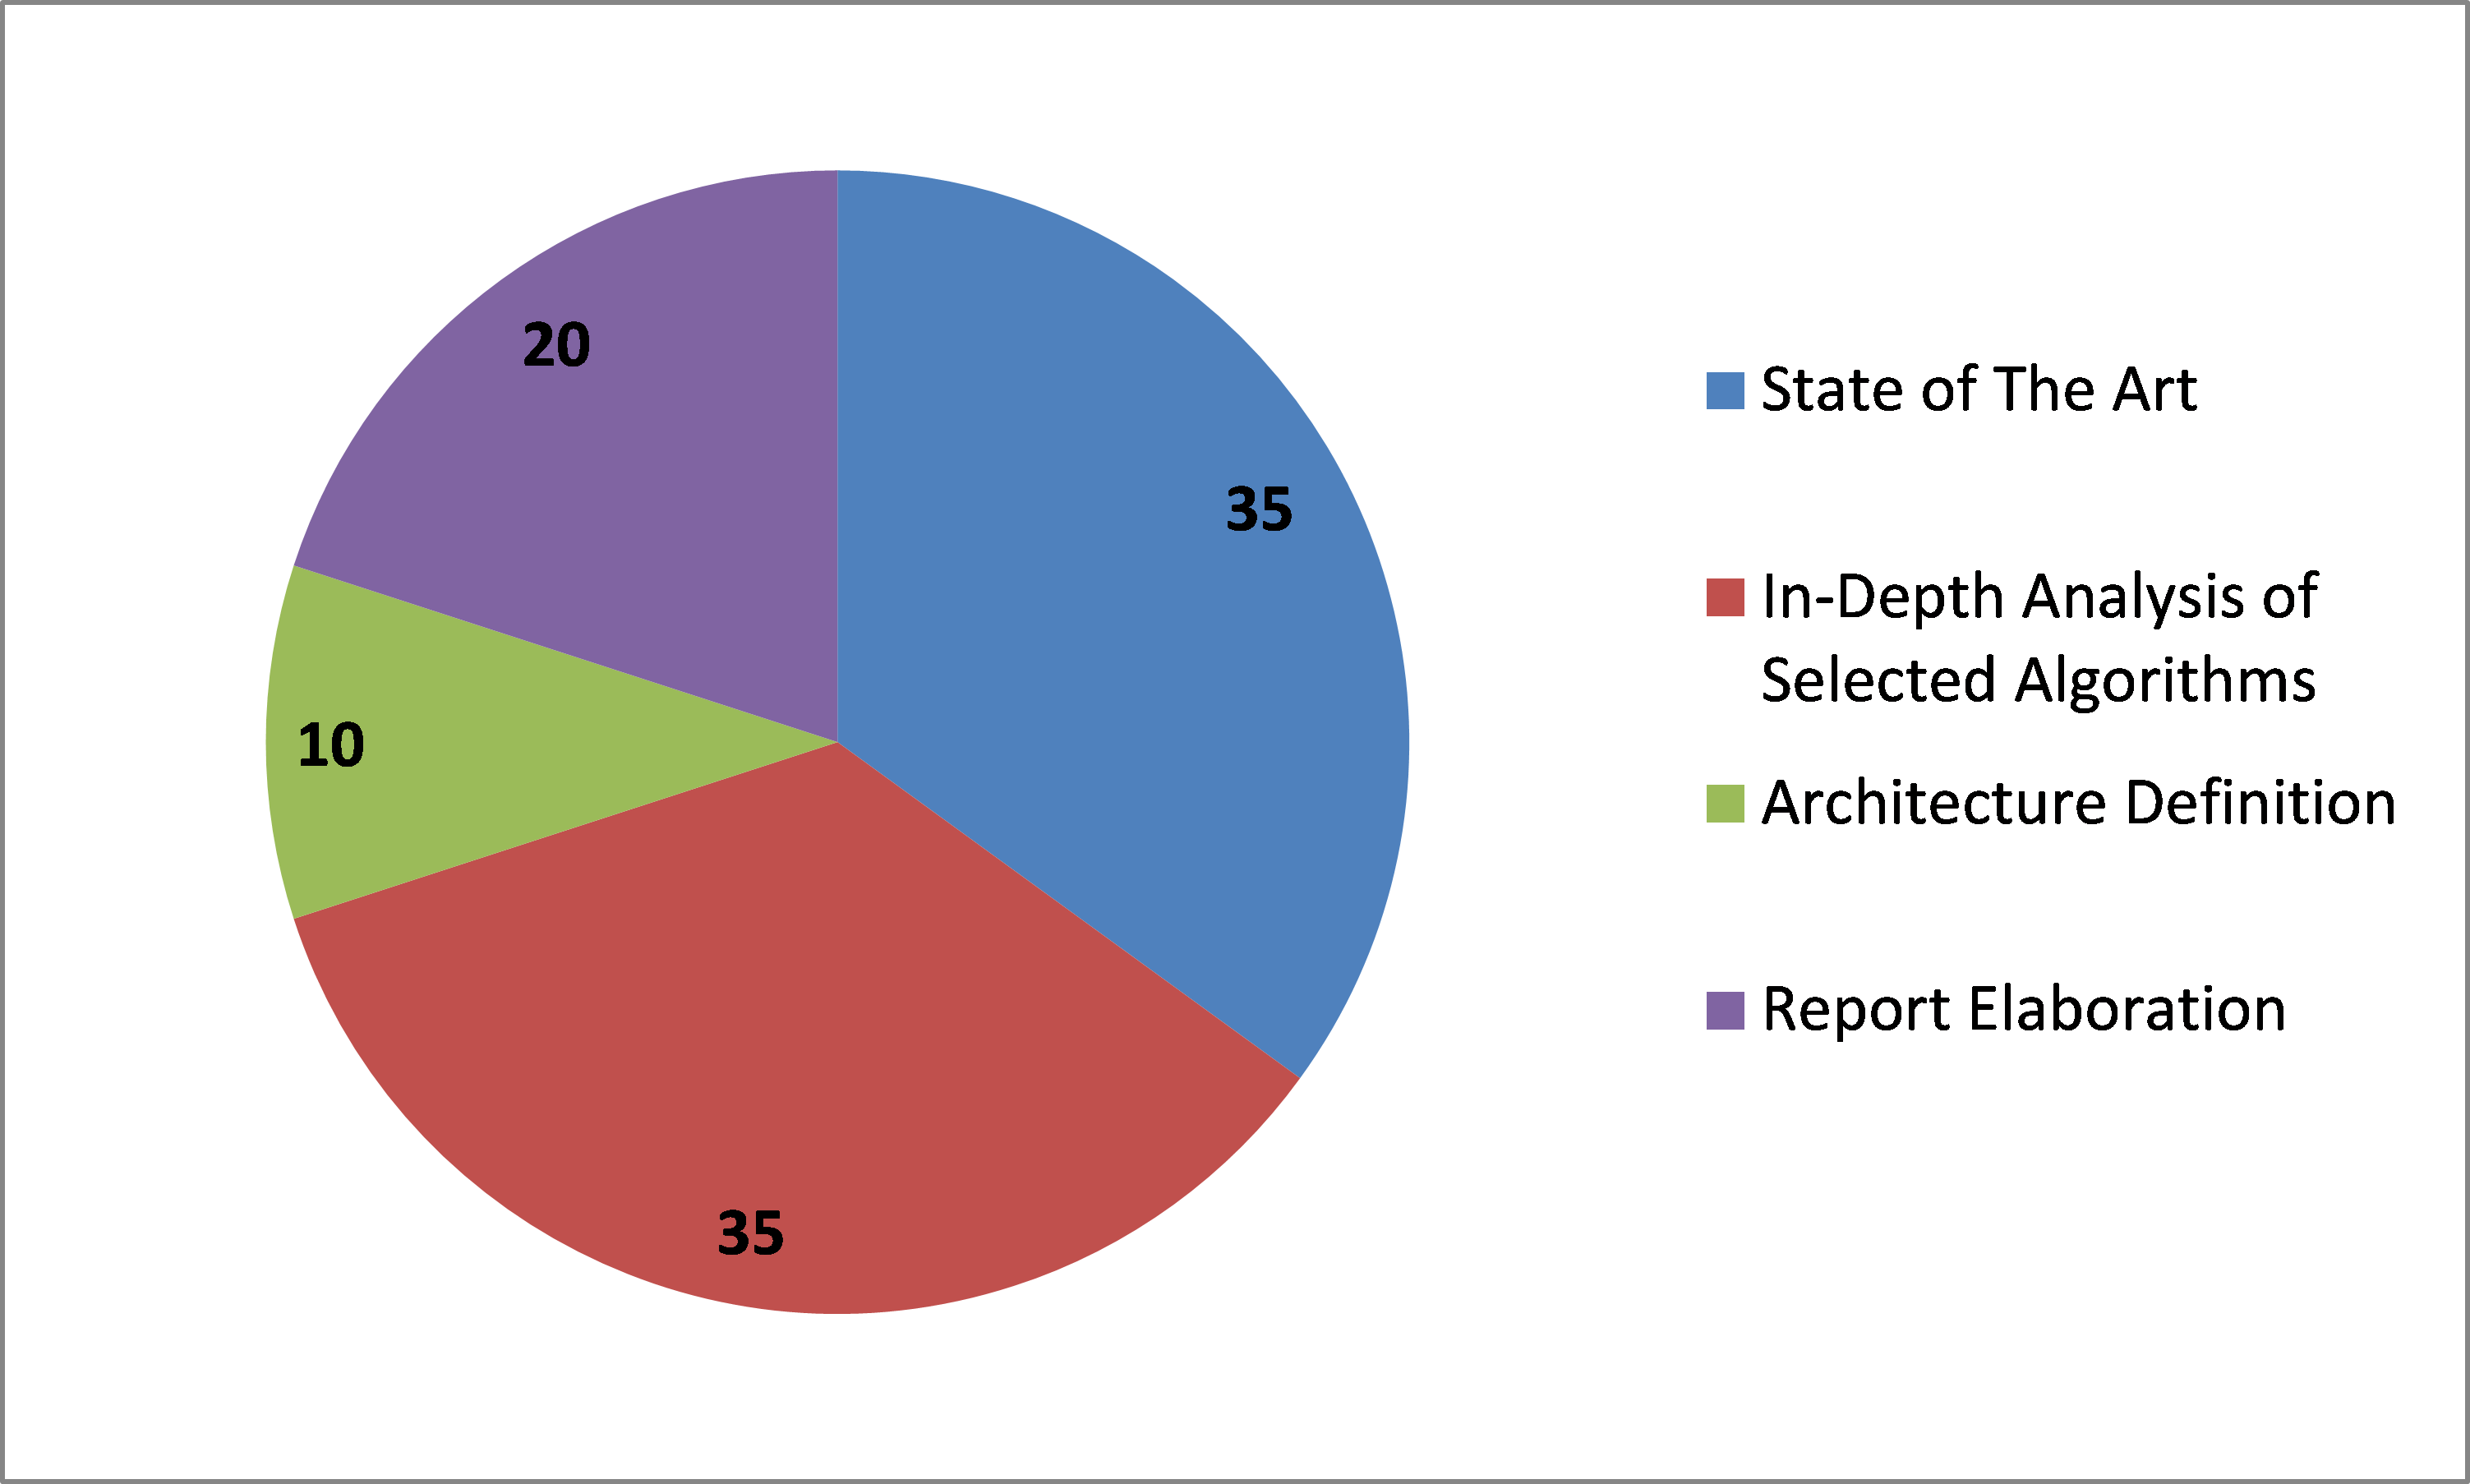
\includegraphics[width=12.72cm]{./images/figures/Fig5_CompletedProjectTasks.png}
   \caption{Allocation of time to the tasks executed in the first phase.}
   \label{fig:ganttDiagram}
\end{figure}\\
The following GANT diagram (Figure~\ref{fig:gantDiagram} ) illustrates a detailed planning for the whole year. It includes all the relevant tasks related to the first and second phases of the project development. The second phase (and pending) tasks are represented in blue.\\
\begin{figure}[h!]
 \centering
   \hspace*{-3,3cm}
   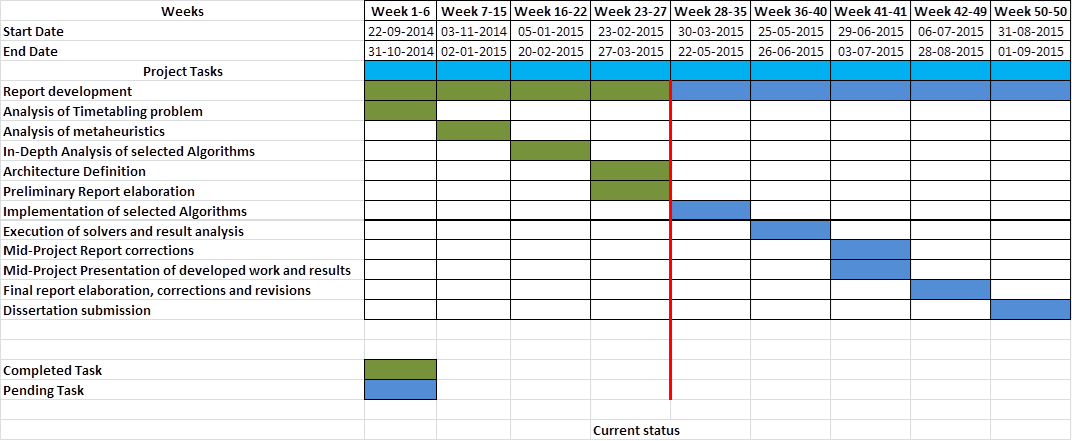
\includegraphics[width=20cm]{./images/figures/Fig6_GANTT_Diagram.png}
   \caption{GANTT diagram detailing the project plan.}
   \label{fig:ganttDiagram}
\end{figure}\\
Some changes to the proposed plan may occur during the project development, influencing the duration and final proposed dates for some tasks may. The time distribution and amount of work to be accomplished between the winter and summer periods is not equally distributed. This is because of the courses taken by the author during the winter semester in parallel with the project development, which consumed a lot of time of the winter period.\\
